\documentclass{article}
\usepackage{indentfirst}
\usepackage{lmodern}
\usepackage[utf8]{inputenc}
\usepackage[T1]{fontenc}
\usepackage[ngerman]{babel}
\usepackage{amssymb,amstext,amsmath}
\usepackage{graphicx}
\usepackage{dsfont}
\usepackage{amsfonts}
\usepackage{graphics}
\usepackage{float}
\usepackage{cite}
\usepackage{url}
\usepackage{tabularx}
\usepackage{capt-of}

\title{Frank-Herz-Versuch}
\author{Alexander Heinisch, Dominik Wille}
\begin{document}
\maketitle

{\begin{center}
\begin{minipage}{\linewidth}
\centering
\makebox[0cm]{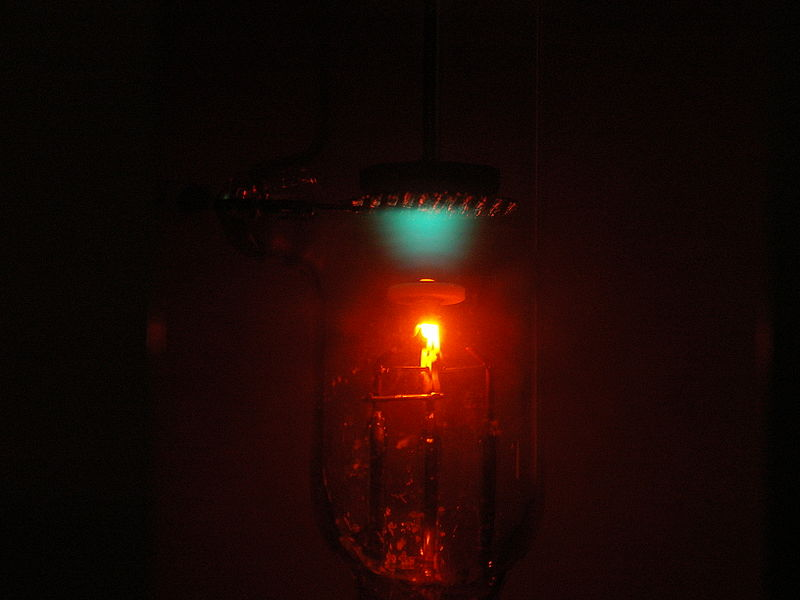
\includegraphics[width=7cm]{bilder/fhz0}}
\label{wtd}
\end{minipage}
\end{center}

\vspace{7cm}
\noindent
\begin{center}
\begin{tabular}{r l}
Tutor & Heimberger\\
Durchführung & 29. Mai 2013 von 14-18 Uhr \\

E-Mail Dominik & dominik.wille@fu-berlin.de \\
E-Mail Alexander & Matthias.Heinisch@gmx.de \\
\end{tabular}
\end{center}

\newpage
\tableofcontents
\newpage

\section{Physikalische Grundlagen}
\subsection{Atommodell}
Am Anfang des 20. Jahrhunderts entdeckten die Physiker James Frank und Gustav Hertz diskrete Anregungsstufen  von Elektronen in Quecksilber. Diese Erkenntnisse waren ein glänzender Beweis für die neue Quantenhypothese und des Bohr-Sommerfeld-Atommodells.\\
In diesem Atommodell nahm Bohr an, dass sich die Elektronen nur auf bestimmten Bahnen strahlungsfrei bewegen können. Dabei entsprechen die Bahnen einem vielfachen der DeBroglie-Wellenlänge (Materiewelle der Elektronen).\\
Demnach können ein Großteil der rechnerischen Bahnen ausgeschlossen werden und es sind nur diskrete Werte für den Drehimpuls und den Bahnradius möglich. Später fand Sommerfeld heraus, dass sich die Elektronen auch auf Ellipsenbahnen bewegen können und nicht nur, wie zuvor angenommen, auf Kreisbahnen. Damit die Bahnen eindeutig parametrisiert werden können, ordnete man ihnen die Quantenzahlen n,l,m,s zu. Dabei beschreibt die Hauptquantenzahl n die Energieniveaus der Elektronen mit den Werten n=1,2,3,... Je größer die Zahl wird, desto weiter ist der Abstand zu dem Kern des Atoms. l ist die Nebenquantenzahl, welche die Exzentrizität der Ellipse im Wertebereich \(o\leq l\leq n-1\). Die Magnetquantenzahl m beschreibt die Ausrichtung der Ellipsen, wodurch die Ellipse nun dreidimensional beschrieben ist. Die Spinquantenzahl s nimmt Werte von \(\pm\frac{1}{2}\) an und beschreibt den Eigendrehimpuls des Elektrons. Durch das Pauli-Prinzip kann nur ein Elektron jeweils ein Energieniveau besetzten.

\subsection{Frank-Hertz-Versuch}
{\begin{center}
\begin{minipage}{\linewidth}
\centering
\makebox[0cm]{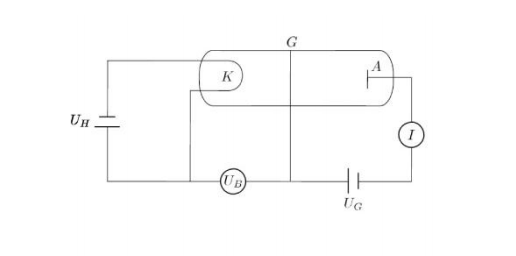
\includegraphics[width=7cm]{bilder/fhz1}}
\captionof{figure}{Versuchsaufbau}%
\label{wtd}
\end{minipage}
\end{center}
Bei Ihrem Experiment hatten sie eine mit Quecksilberdampf gefüllte Röhre, in welcher Elektronen von einer Glühkathode K aus beschleunigt werden und durch ein Gitter G zu einer Auffangelektrode A gelangen. Die Beschleunigung erfolg mithilfe einer Heizspannung \(U_H\). Sie ist bedeutend größer als die zwischen dem Gitter und der Anode anliegenden Bremsspannung \(U_G\)\\
Anfangs erfolgen nur elastische Stöße der Elektronen mit dem Quecksilber und im Auffängerkreis ist eine gleichmäßig zunehmender Stromfluss messbar. Erreicht die Beschleunigungsspannung jedoch einen Schwellenwert bzw. ihr ganzzahliges Vielfaches, so bricht der Strom ab und steigt anschließend wieder von neuem an.\\
Im Praktikum werden wir Bariumoxidkathoden benutzen und die in der Röhre angeordneten Elektroden sind planparallel angeordnet. Der Abstand zwischen Kathode und Anode ist größer als die mittlere freie Wellenlänge, wodurch die Stoßwahrscheinlichkeit erhöht wird.

\section{Aufgaben}
\subsection{Aufgabe 1}
Beobachtung der Elektronenstoß-Anregungskurve (Frank-Hertz-Kurve) von Quecksilber bei einer (Ofen-)Temperatur von etwa 19\(^\circ\)C mit dem Oszilloskop. Optimierung der Kurve durch geeignete Einstellungen der experimentellen Parameter (Ofenheizung, Kathodenheizung, Beschleunigungsspannung)

\subsection{Aufgabe 2}
Quantitative Aufnahme der Kurve mit einem X-Y-Schreiber. Bestimmung der zugehörigen Übergangsenergie in Quecksilber.

\subsection{Aufgabe 3}
Beobachtung und Registrierung weiterer Anregungskurven für Temperaturen von 150 und 210\(^\circ\)C. Qualitative Diskussion der Ergebnisse.

\subsection{Aufgabe 4}
Aufnahme und Auswertung einer Frank-Hertz-Kurve für Neon bei Zimmertemperatur.
\end{document}